\chapter{User Interfaces}

So far we have worked hard on the core mechanic of our game. Another important
aspect are the screens and components that wrap this mechanic. In this chapter
you will learn how to implement menus, popups and other user interface elements
in \cocos{}. 

\cocos{} provides its own set of basic UI components, such as buttons and
labels. For most games these components are sufficient. However, in this chapter
we also learn how to integrate Apple's UI framework \textit{UIKit}. Knowing
that is important for integrating many core Apple API's. As a specific example,
we will add integrate the Game Center framework in this chapter.

By the end of this chapter we will have a fully functional game!
Here's the basic screen flow our game will have:

\begin{figure}[H]
		\centering
		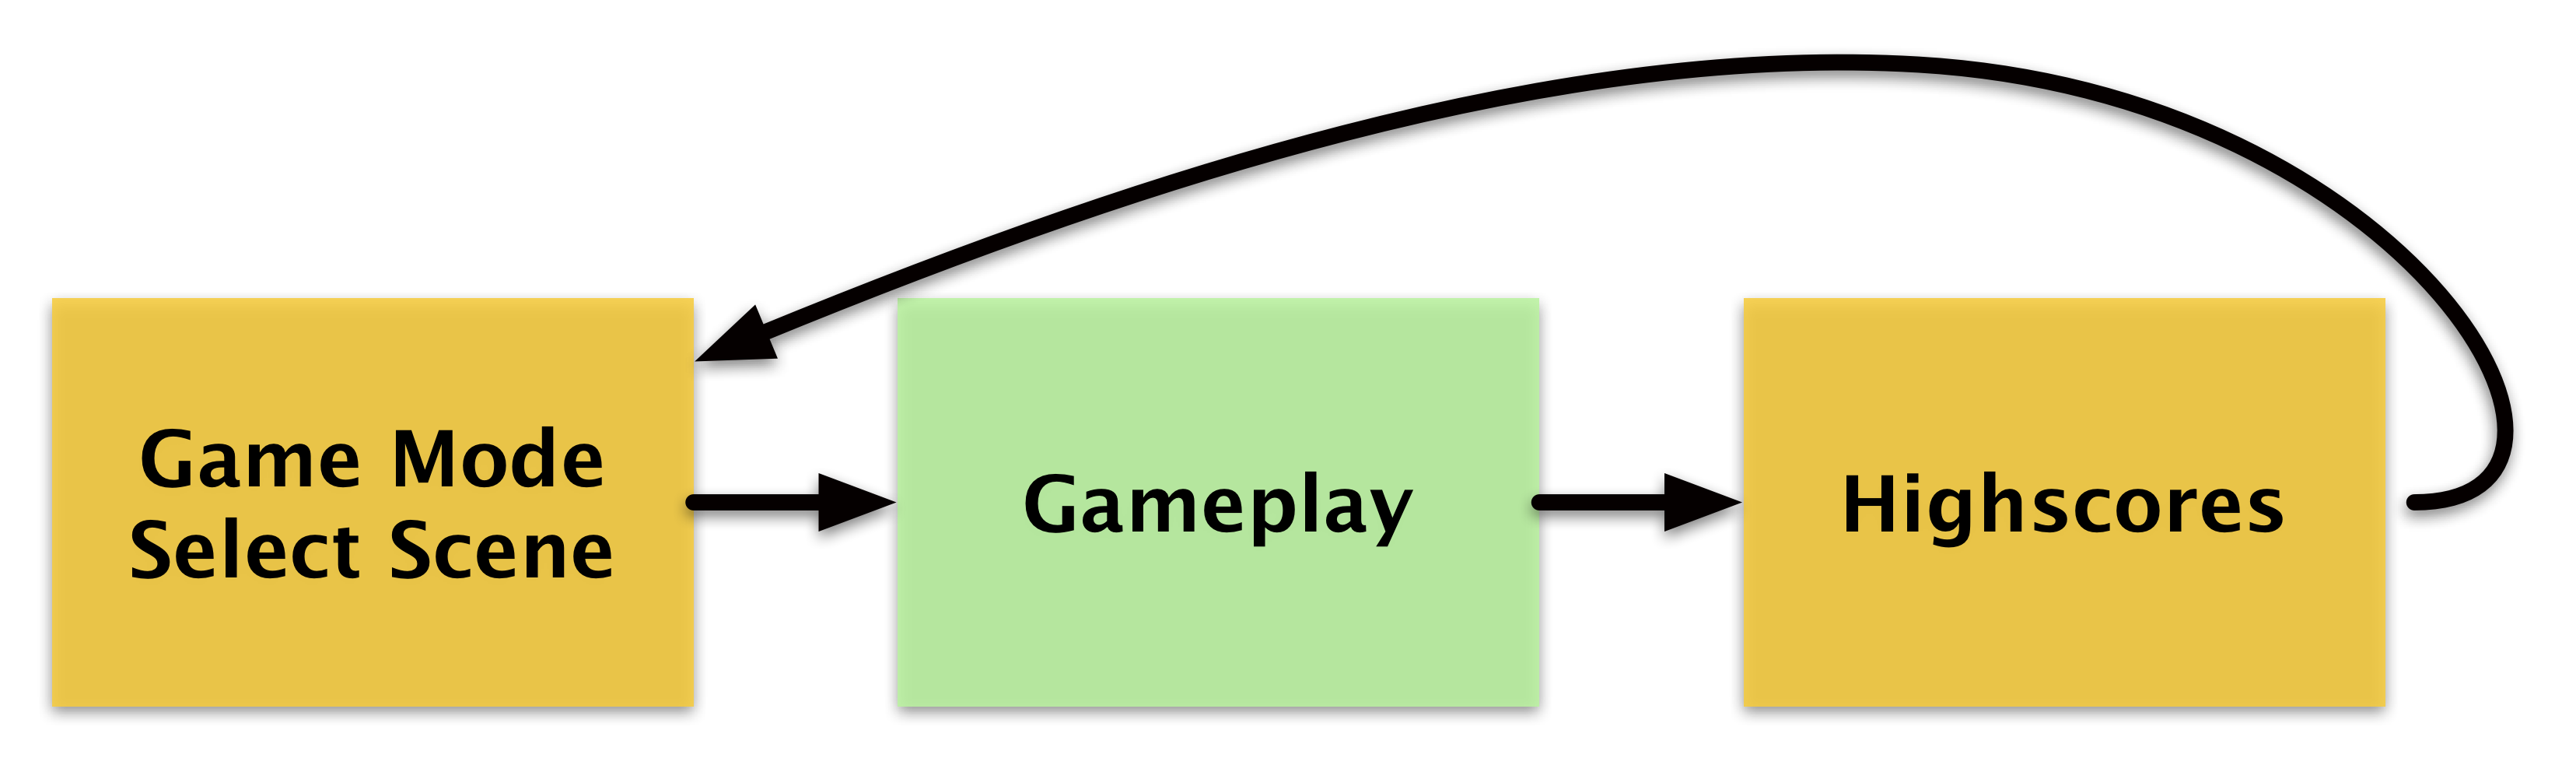
\includegraphics[width=0.7\linewidth]{images/Chapter6/screen_flow.png}
\end{figure}

Let's start out by adding the game mode scene!

\section{Adding a game mode selection scene}
